\section{Introduction}\label{sec:intro} 

Compilation of programs for distributed memory architectures using message passing is a vital task with potential for speedups over existing techniques. The partitioned global address space (PGAS) parallel programming model automates the production of message passing code from a shared memory programming model and exposes locality of reference information to the programmer thereby improving programmability and allowing for compile-time performance optimizations. In particular, programs compiled to message passing hardware can improve in performance by aggregating messages and eliminating dynamic locality checks for affine array accesses in the PGAS model. 

Message passing code generation is a difficult task for an optimizing compiler targeting a distributed memory architecture. These architectures are comprised of independent units of computation called locales. Each locale has its own set of processors, cores, memory, and address space. For programs executed on these architectures, data is distributed across various locales of the system, and the compiler needs to reason about locality in order to determine whether a program data access is remote (requiring a message to another locale to request a data element) or local (requiring no message and accessing the data element on the locale's own memory). Only a compiler with sufficient knowledge about locality can compile a program in this way with good communication performance. 

Each remote data memory access results in a message with some non-trivial run time overhead, which can drastically slow down a program's execution time. This overhead is caused by latency on the interconnection network and locality checks for each data element. Accessing multiple remote data elements individually results in this run time overhead being incurred multiple times, whereas if they are transferred in bulk the overhead is only incurred once. Therefore, aggregating messages improves performance of message passing codes. In order to transfer remote data elements in bulk, the compiler must be sure that all elements in question are remote before the message is sent. 

The vast majority of loops in scientific programs access data using affine array accesses. An affine array access is one whose indices are linear combinations of the loop's induction variables. For example, for a loop with induction variables $i$ and $j$, accesses $A[i, j]$ and $A[2i-3, j+1]$ are affine, but $A[i^2]$ is not. Loops using affine array accesses are special because they exhibit regular access patterns within a data distribution. Compilers can use this information to decide when message aggregation can take place. 

\begin{comment}
Although a simple concept to understand, message aggregation is the most complicated part of message passing code generation. Existing methods \cite{goumas2006message, xue1997communication} split the loop iteration space into tiles (also known as footprints) of consecutive iterations, and each locale executes its tile's iterations in parallel. Communication using aggregation takes place between locales just before and after the computation within a single tile. These methods require the compiler to do complex footprint calculations, optimizing for tile size and shape, before message aggregation can take place. As \cite{ramanujam1992tiling} shows, determining tile shape quickly becomes difficult for more complicated loop structures, since the optimum tile shape for a computation is not always rectangular. It is our belief that message aggregation using tiling is not used in production quality compilers today because of the complexity of message aggregation calculations, described above. What is needed is a simple, robust, and widely applicable method for message aggregation that leads to improvements in performance. 
\end{comment}

Broadly speaking all have the following steps:

\begin{itemize}

\item {\bf Loop distribution} The loop iteration space for each nested loop is divided into portions to be executed on each locale (message passing node), called iteration space tiles. 

\item {\bf Data distribution} The data space for each array is distributed according to the directive of the programmer (usually as block, cyclic, or block-cyclic distributions.)

\item {\bf Footprint calculation} For each iteration space tile, the portion of data it accesses for each array reference is calculated as a formula on the symbolic iteration space bounds. This is called the data footprint of that array access.

\item {\bf Message aggregation calculation} For each array access, its data footprint is intersected with each possible locale's data tile to derive symbolic expressions for the bounds of the polyhedron in the data space for the portion of the data footprint that intersects with the locale's data tile. This portion of the data tile for locales other than the loop tile's locale needs to be communicated remotely from that data tile's locale to the loop tile's locale.

\end{itemize}

It is the message aggregation calculation step above that reveals the portion of data to be aggregated for communication. Unfortunately, of the steps above, message aggregation calculation is by far the most complex. Loop distribution and data distribution are straightforward; footprint calculation is of moderate complexity using matrix formulations; but it is message aggregation calculation that defies easy mathematical characterization for the general case of affine accesses. Instead some very complex research methods \cite{goumas2006message, xue1997communication} have been devised that make many simplifying assumptions on the types of affine accesses supported, and yet remain so complex that they are rarely implemented in production compilers.

Although the steps above are primarily for traditional methods of parallel code generation, polyhedral methods dont fare much better. Polyhedral methods have powerful mathematical formulations for loop transformation discovery, automatic parallelization, and parallelism coarsening. However message aggregation calculation is still needed but not modeled well in polyhedral models, leading to less capable ad-hoc methods for it.

It is our belief that message aggregation using tiling is not used in production quality compilers today because of the complexity of message aggregation calculations, described above. What is needed is a simple, robust, and widely applicable method for message aggregation that leads to improvements in performance. 

This paper presents a loop optimization for message passing code generation based on a technique called modulo unrolling. Using modulo unrolling, the locality of any affine array access can be deduced at compile time if the data is distributed in a cyclic or block cyclic fashion. The optimization can be performed by a compiler to aggregate messages and reduce a program's execution time and communication. 

Modulo unrolling in its original form, pioneered by \cite{barua1999maps}, was meant to target tiled architectures such as the MIT Raw machine, not distributed memory architectures that use message passing. It has since been modified to apply to such machines in this work. Modulo unrolling works as follows. It its basic form, it unrolls each affine loop by a factor equal to the number of locales of the machine being utilized by the program. If the arrays used in the loop are distributed cyclically or block cyclically, each array access is guaranteed reside on a single locale across all iterations of the loop. Using this information, the compiler can then aggregate all remote array accesses that reside on a remote locale into a single message before the loop. If remote array elements are written to during the loop, one message is required to store these elements back to each remote locale after the loop runs. 

We build on the modulo unrolling method to solve the very difficult problem of message aggregation in message passing machines. Chapel is an explicitly parallel programming language developed by Cray Inc. that falls under the Partitioned Global Address Space (PGAS) memory model. Here, a system's memory is abstracted to a single global address space regardless of the hardware architecture and is then logically divided per locale and thread of execution. By doing so, locality of reference can easily be exploited no matter how the system architecture is organized. The Chapel compiler is an open source project used by many in industry and academic settings. The language contains many high level features such as zippered iteration, leader and follower iterator semantics, and array slicing that greatly simplify the implementation of modulo unrolling into the language.

Although our method is described in the context of Chapel, it is adaptable to any PGAS language. However, for other languages the implementation may differ. For example, if the language does not use leader and follower iterator semantics to implement parallel for loops, the changes to those Chapel modules that we present here will have to be implemented elsewhere in the other PGAS language where parallel for loop functionality is implemented.

\subsection{Chapel's Data Distributions} 

In this work, we consider three types of data distributions: Block, Cyclic, and Block Cyclic. In a Block distribution, elements of an array are mapped to locales evenly in a dense manner. In a Cyclic distribution, elements of an array are mapped in a round-robin manner across locales. In a Block Cyclic distribution, a number of elements specified by a block size parameter is allocated to consecutive array indices in a round robin fashion. Figures \ref{block_dist} - \ref{cyc_dist} illustrate these three Chapel distributions for a two-dimensional array, whose data space is shown. In Figure \ref{block_cyc_dist}, the array takes a 2 x 2 block size parameter. 

The choice of data distribution to use for a program boils down to computation and communication efficiency. Different programs and architectures may require different data distributions. It has been shown that finding an optimal data distribution for parallel processing applications is an NP-complete problem, even for one or two dimensional arrays \cite{mace1987memory}. Certain program data access patterns will result in fewer communication calls if the data is distributed in a particular way. For example, many loops in stencil programs that contain nearest neighbor computation will have better communication performance if the data is distributed using a Block distribution. This occurs because on a given loop iteration, the elements accessed are near each other in the array and therefore more likely to reside on the same locale block. Accessing elements on the same block does not require a remote data access and can be done faster. However, programs that access array elements far away from each other will have better communication performance if data is distributed using a Cyclic distribution. Here, a Block distribution is almost guaranteed to have poor performance because the farther away accessed elements are the more likely they reside on different locales. 

A programmer may choose a particular data distribution for reasons unknown to the compiler. These reasons may not even take communication behavior into account. For example, Cyclic and Block Cyclic distributions provide better load balancing of data across locales than a Block distribution because elements can be added or removed according to a regular predictable pattern. In many applications, data redistribution may be needed if elements of a data set are inserted or deleted at the end of the array. In particular, algorithms to redistribute data using a new block size exist for the Block Cyclic distribution \cite{walker1996redistribution, prylli1997fast}. If an application uses a dynamic data set with elements being appended, a Cyclic or Block Cyclic distribution is superior to Block because new elements are added to the locale that follows the cyclic or block cyclic pattern. For Block, the entire data set would need to be redistributed every time a new element is appended, which can be expensive. 

Compatibility with other PGAS languages might be an important consideration for a programmer when selecting a data distribution. Data sets used by Chapel programs and other PGAS programs should use Cyclic or Block Cyclic distributions because other PGAS languages do not support the Block distribution. A programmer would benefit by distributing the same data set using only one scheme so the data would not have to be replicated for different programs. This is an important consideration for vast data sets which have already been distributed on message passing computers, and we want to perform additional computation on them, perhaps with other programs.  

Therefore, in this work, it is our view that the compiler should not change the programmer's choice of data distribution in order to achieve better runtime and communication performance. The compiler should attempt to perform optimizations based on the data distribution that the programmer specified. Our optimization is meant to be applied whenever the programmer specifies a Cyclic or Block Cyclic distribution. It is not applied when the programmer specifies a Block distribution.

\begin{figure}
	\begin{center}
	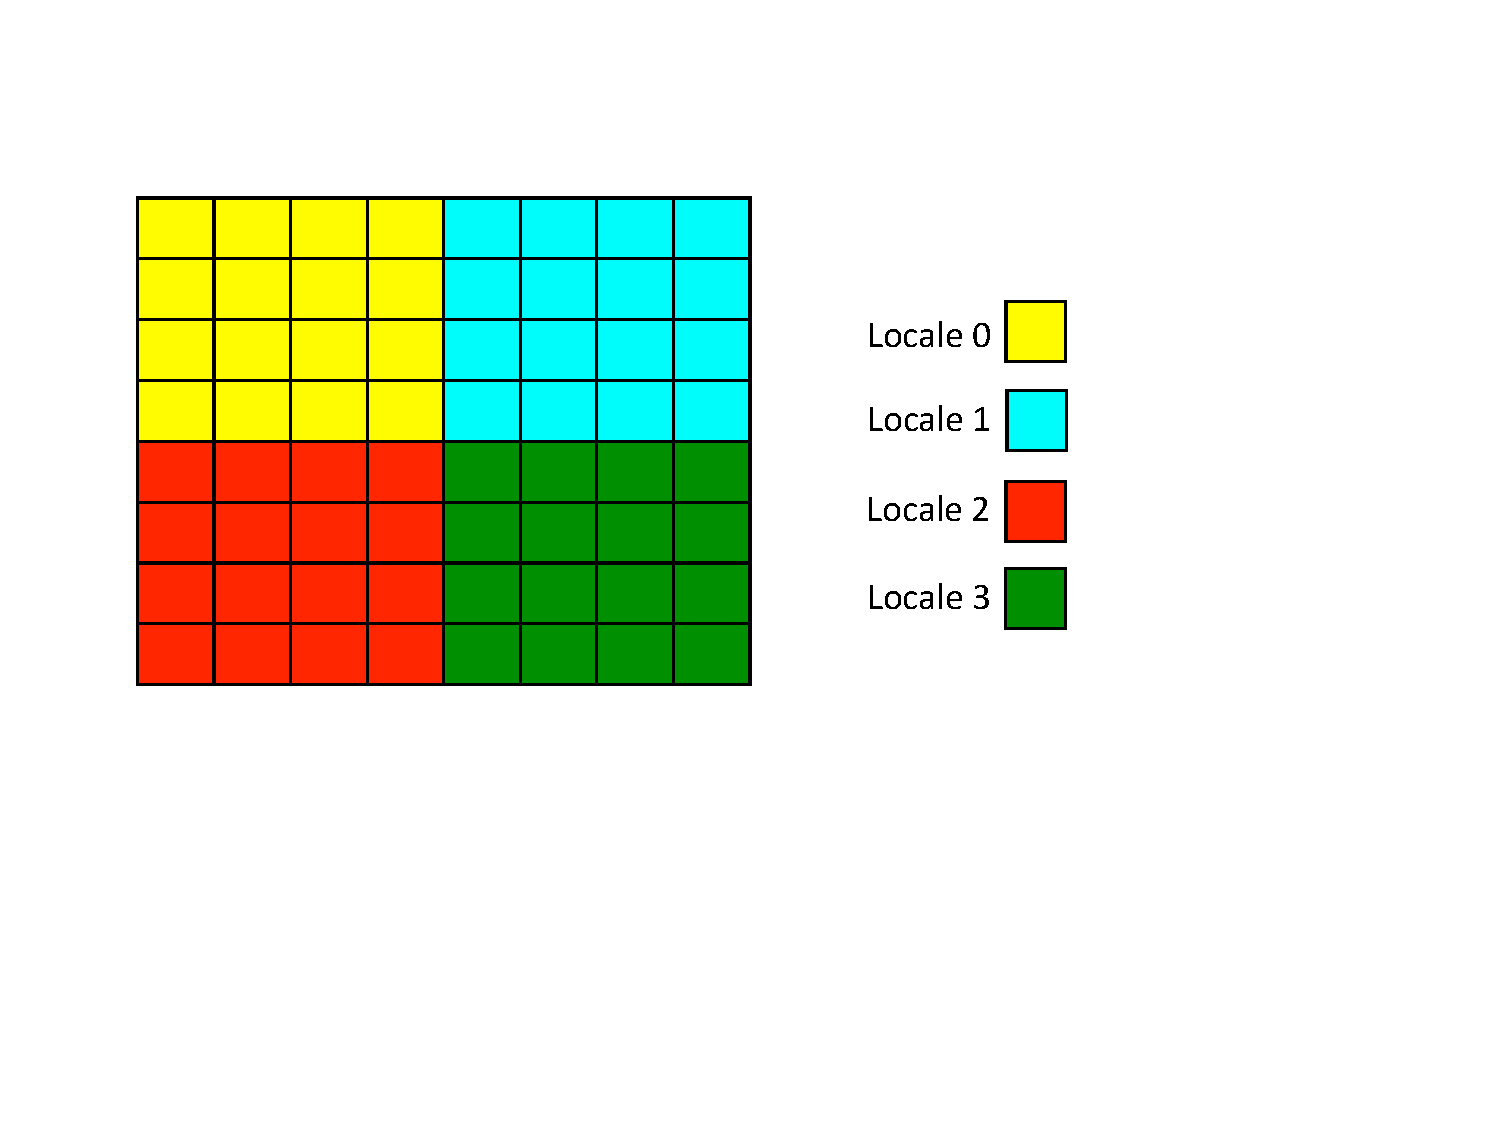
\includegraphics[scale=0.55]{./Figures/block_dist}
	\caption{Chapel Block distribution.}
	\label{block_dist}
	\end{center}
\end{figure}

\begin{figure}
	\begin{center}
	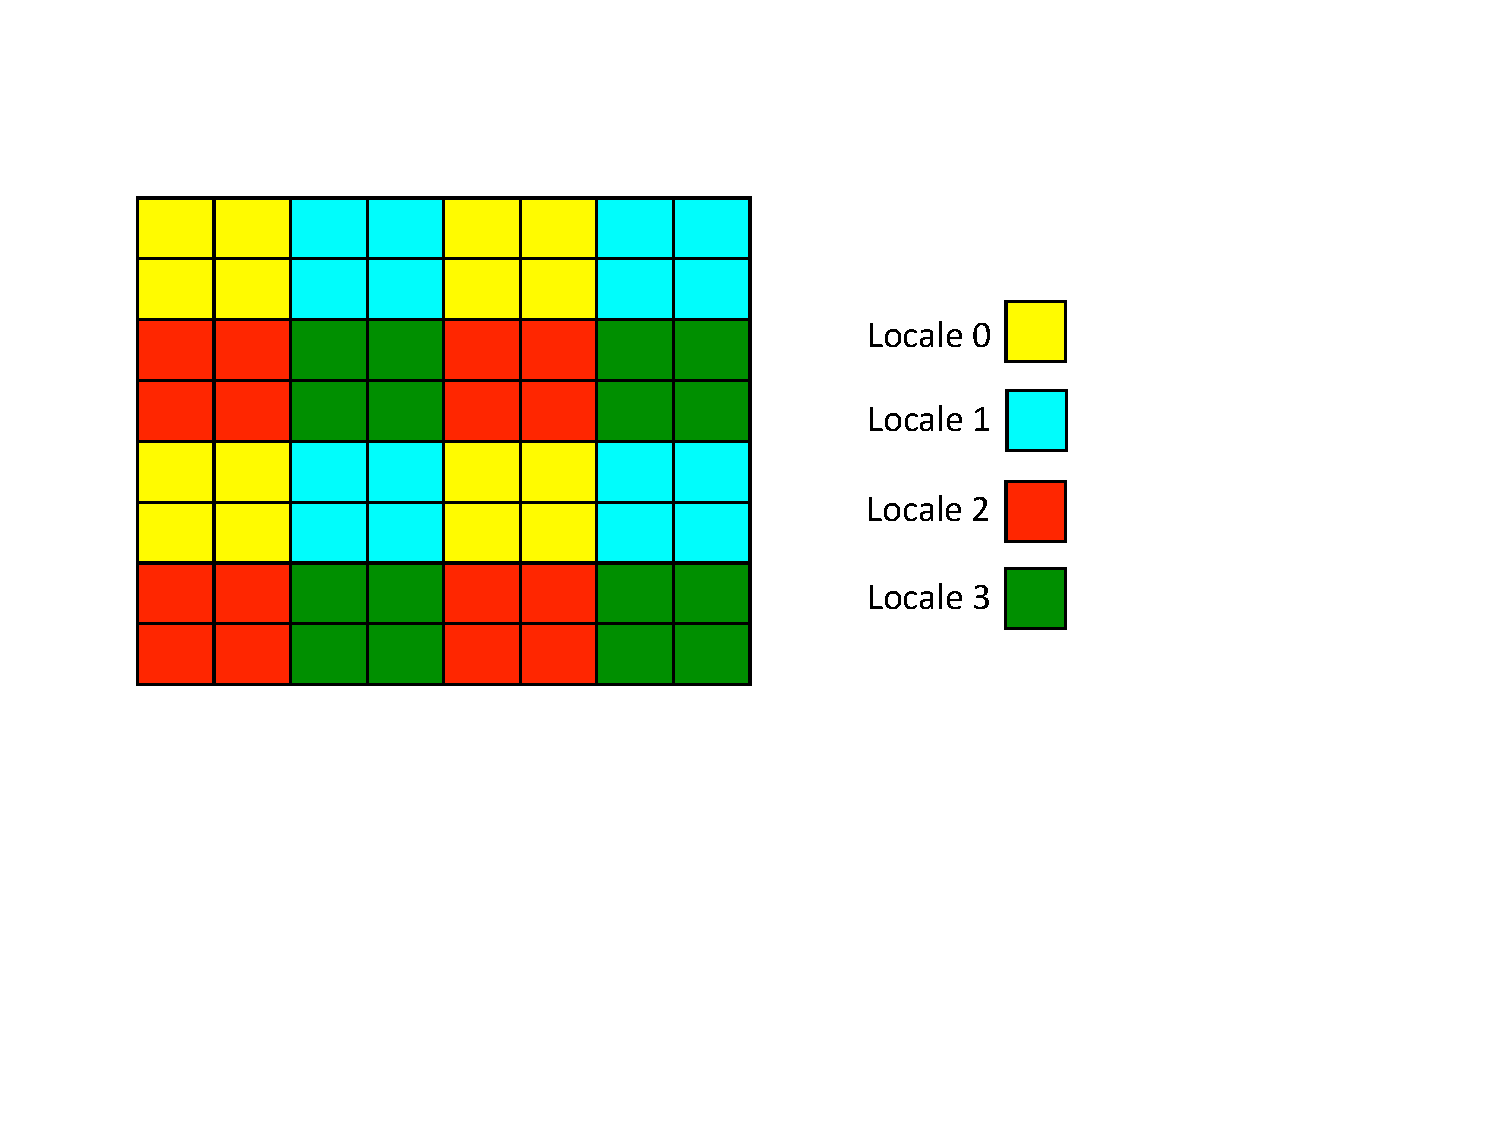
\includegraphics[scale=0.55]{./Figures/block_cyc_dist}
	\caption{Chapel Block Cyclic distribution with a 2 x 2 blocksize parameter.}
	\label{block_cyc_dist}
	\end{center}
\end{figure}

\begin{figure}
	\begin{center}
	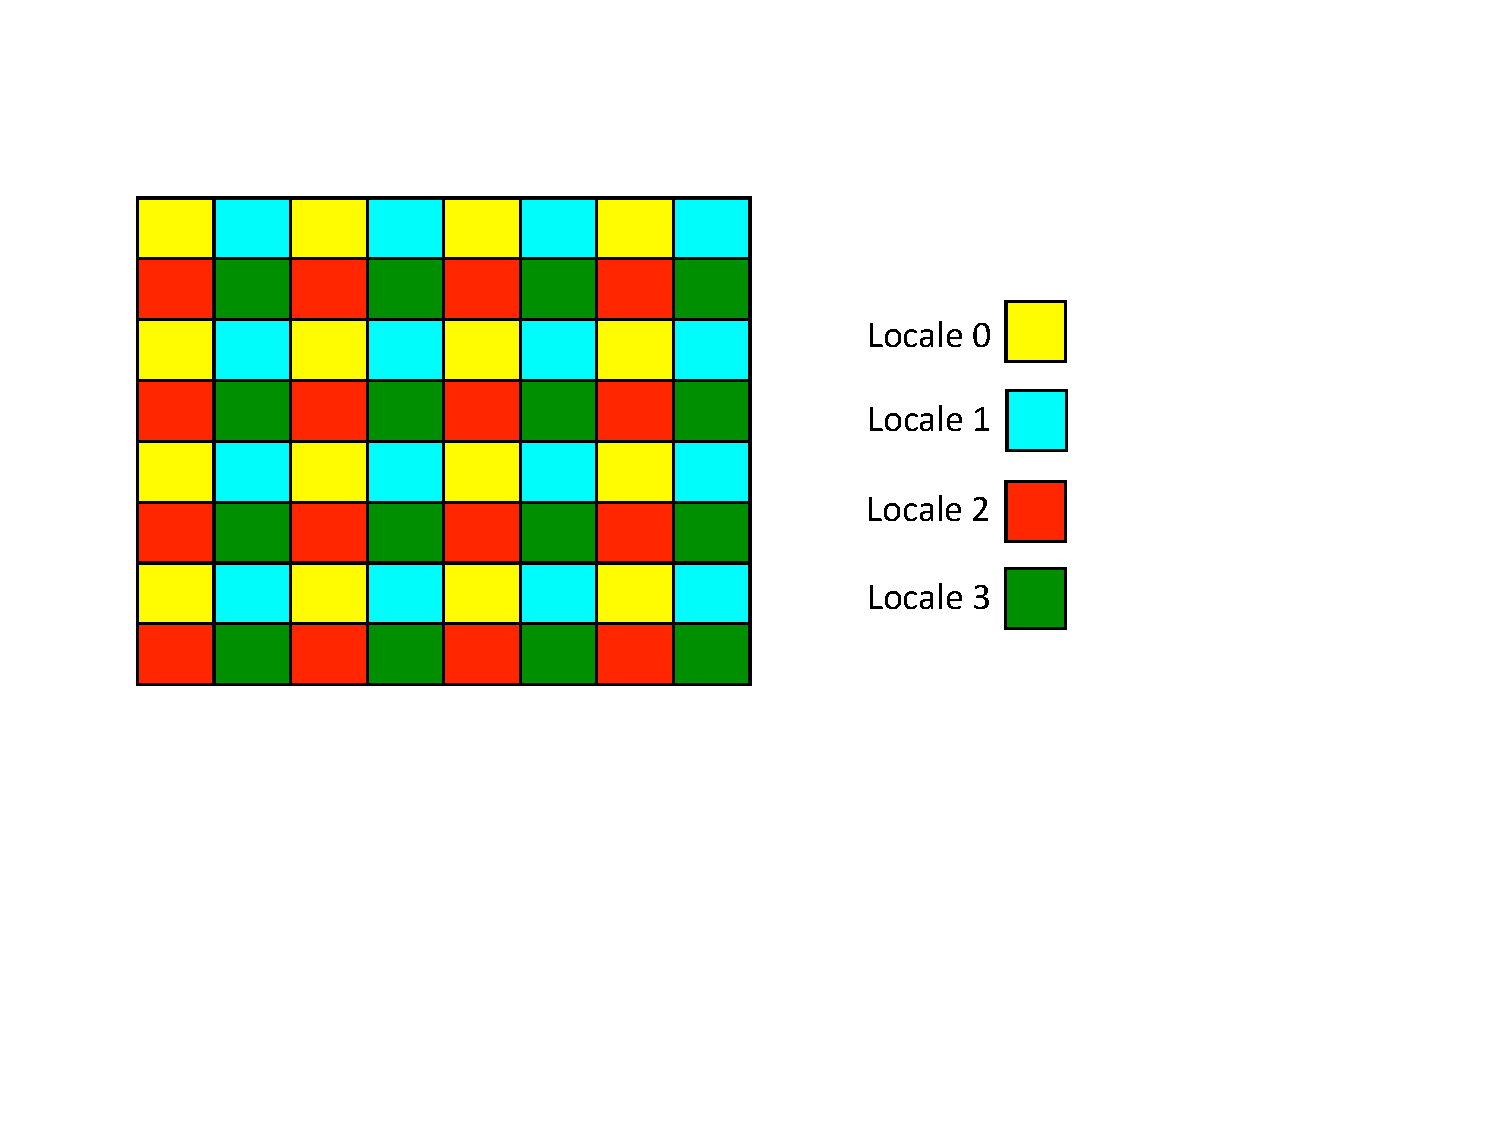
\includegraphics[scale=0.55]{./Figures/cyc_dist}
	\caption{Chapel Cyclic distribution.}
	\label{cyc_dist}
	\end{center}
\end{figure}



